\documentclass[12pt]{article}
\usepackage{scrextend}
\usepackage[utf8]{inputenc}
\usepackage[polish]{babel}
\usepackage[T1]{fontenc}%polskie znaki
\usepackage[utf8]{inputenc}%polskie znaki
\usepackage{geometry}
\usepackage{float}
\usepackage{enumitem}
\usepackage{hyperref}
\usepackage{graphicx}
\usepackage{amsmath}

\renewcommand{\baselinestretch}{1.5}


\begin{document}

\begin{flushleft}
    Damian Koper \textbf{241292} \\
\end{flushleft}
\vspace{1cm}
{
    \centering
    {\Huge\scshape\bfseries Modelowanie i analiza systemów informatycznych }\\
    \large{Sieci Petriego - konstrukcja i analiza behawioralna sieci Petriego}\\
    \vspace{0.5cm}
}
\newcounter{ex}
\setcounter{ex}{0}
\newcommand{\ex}[1]{
    \refstepcounter{ex}{
        \noindent\normalfont\Large\bfseries Zadanie \arabic{ex}.
    } \\
    #1
}

\ex{Formalny opis sieci}
\vspace{-0.5cm}

\begin{figure}[H]
    \centering
    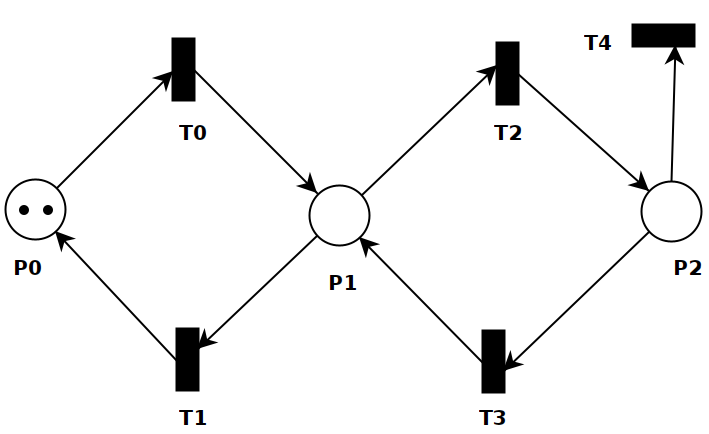
\includegraphics[width=0.5\linewidth]{../../lab6/ex_1}
    \caption{Opisywana sieć}
\end{figure}
\vspace{-1cm}
\begin{align*}
    SP  & = \langle{P,T,F,H,W,C,M_0}\rangle                         \\
    P   & =\{p_0, p_1, p_2\}                                        \\
    T   & =\{t_0, t_1, t_2, t_3, t_4\}                              \\
    F   & = \{\{p_0, t_0\},\{t_0, p_1\},\{p_1,t_1\},\{t_1,p_0\}\,
    \{p_1, t_2\},\{t_2, p_2\},\{p_2,t_3\},\{t_3,p_1\},\{p_2,t_4\}\} \\
    H   & = \emptyset                                               \\
    W   & = \{1,1,1,1,1,1,1,1,1\}                                   \\
    C   & = \{\infty,\infty,\infty\}                                \\
    M_0 & =\{2,0,0\}
\end{align*}
\newpage

\ex{Graf osiągalności}
\begin{figure}[h]
    \centering
    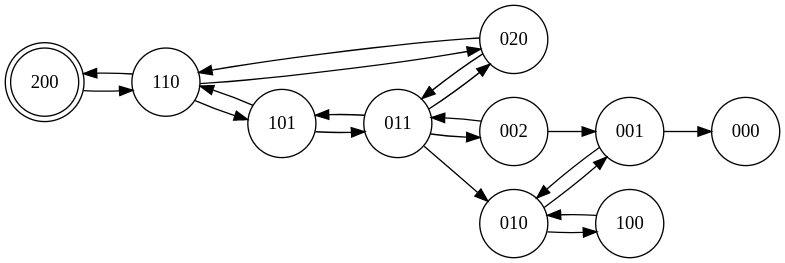
\includegraphics[width=\linewidth]{../../lab6/graph.dot.png}
    \caption{Graf osiągalności sieci z zadania 1}
\end{figure}

\ex{Analiza behavioralna}

\begin{itemize}[noitemsep]
    \item Sieć jest 2-ograniczona -- w jedym momencie w każdym miejscu mogą przebywać maksymalnie 2 znaczniki.
    \item Sieć nie jest bezpieczna -- nie jest 1-ograniczona.
    \item Sień nie jest zachowawcza -- jej znaczniki mogą być usuwane poprzez przejście~$t_4$.
    \item Sieć nie jest żywotna -- nie można odpalić żadnego przejścia jesli sieć osiągnie stan $(000)$.
    \item Sieć nie jest odwracalna -- stany z liczbą znaczników 2 nie są osiągalne po usunięciu znacznika poprzez przejście $t_4$.
    \item Sieć nie jest trwała -- w stanach $(011)$ i $(110)$ nie można na raz odpalić przejścia $t_1$ i $t_2$.
\end{itemize}

\newpage

\ex{Rozbudowa sieci}

\begin{figure}[h]
    \centering
    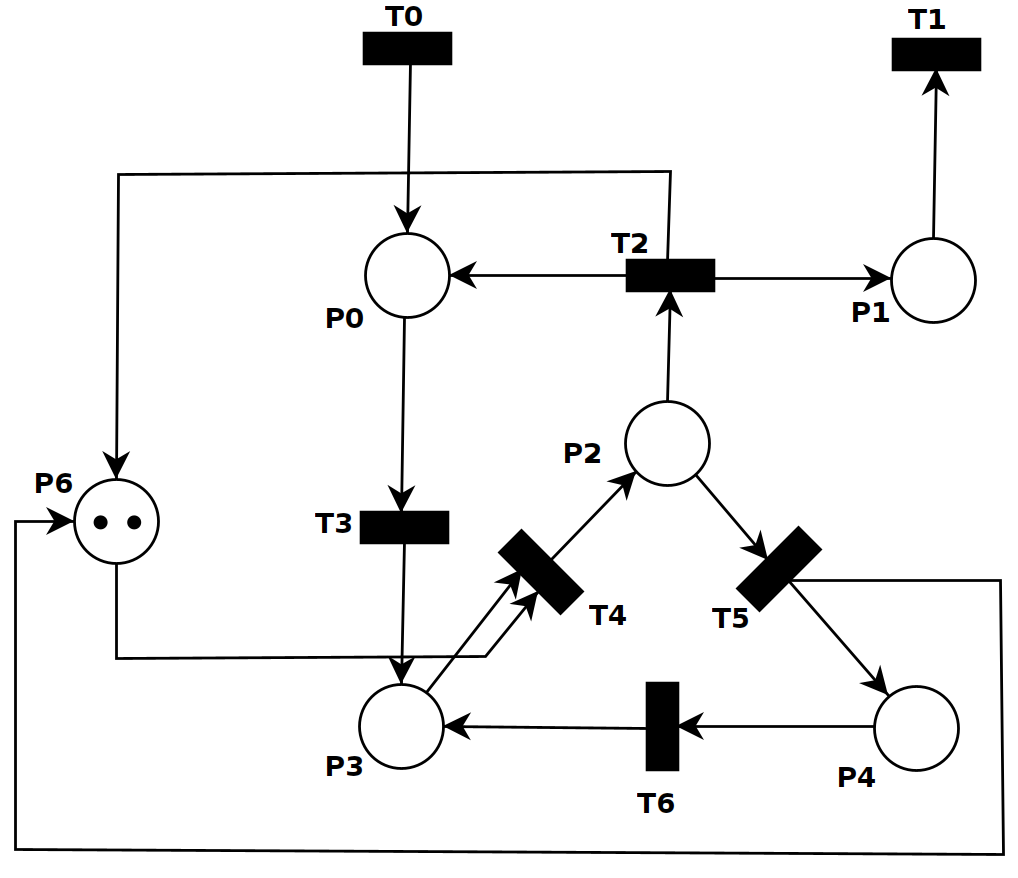
\includegraphics[width=0.8\linewidth]{../../lab6/ex_4}
    \caption{Rozbudowana sieć z ograniczeniem liczby znaczników w $p_2$.}
\end{figure}


\end{document}

wyzna
